\documentclass[conference]{IEEEtran}
\IEEEoverridecommandlockouts

\usepackage[utf8]{inputenc}
\usepackage[T1]{fontenc}
\usepackage[brazil]{babel}
\usepackage{cite}
\usepackage{amsmath,amssymb}
\usepackage{graphicx}
\usepackage{booktabs}
\usepackage{url}
\usepackage{xcolor}
\usepackage[hidelinks]{hyperref}
\graphicspath{{figuras/}}

\begin{document}

\title{Exploração Visual da Cobertura Midiática das Eleições Brasileiras de 2026 com o GDELT Global Knowledge Graph}

\author{\IEEEauthorblockN{[Nome do(a) aluno(a)]}
\IEEEauthorblockA{\textit{[Disciplina] --- [Instituição]}\\
[Cidade], Brasil \\
[e-mail]}}

\maketitle

\begin{abstract}
Este trabalho apresenta a exploração visual de 95.403 notícias sobre as eleições gerais brasileiras de 2026, publicadas entre 1º e 30 de outubro de 2026 e indexadas pelo \emph{Global Knowledge Graph} (GKG 2.0) do projeto GDELT. Foi construído um painel interativo em Python (Streamlit e Plotly) que integra séries temporais, mapas de calor, mapa de símbolos proporcionais, grafo de coocorrência e tabelas coordenadas por um único conjunto de filtros. A exploração revelou, primeiro, um artefato de coleta: 13.423 páginas geradas automaticamente com resultados por seção eleitoral, que inflavam o volume e o tom positivo da cobertura. Revelou também uma sub-detecção sistemática do nome ``Lula'' pelo reconhecedor de entidades do GDELT. Após o tratamento desses problemas, observou-se que a mídia internacional é consistentemente mais negativa que a nacional (tom médio $-1{,}58$ contra $-0{,}45$; $d$ de Cohen $=0{,}45$). Os picos de atenção coincidem com os dois turnos, e após o segundo turno a agenda se desloca para corrupção, fraude eleitoral e judicialização, impulsionada sobretudo pela imprensa estrangeira.
\end{abstract}

\begin{IEEEkeywords}
visualização de informação, análise exploratória visual, GDELT, eleições, análise de mídia, dashboards interativos
\end{IEEEkeywords}

%==============================================================
\section{Introdução}
%==============================================================
A \emph{visualização de informação} estuda representações visuais interativas de dados abstratos que ampliam a cognição humana~\cite{card1999,munzner2014}. Na \emph{análise exploratória visual}, o usuário não parte de hipóteses fechadas. Ele as formula e refina enquanto interage com as representações, alternando entre visões gerais e detalhes~\cite{shneiderman1996,keim2002}. Essa abordagem é especialmente útil quando os dados são volumosos, heterogêneos e ruidosos, como os gerados automaticamente a partir de notícias.

O projeto GDELT (\emph{Global Database of Events, Language, and Tone}) monitora continuamente notícias da imprensa mundial em mais de 100 idiomas e extrai delas temas, pessoas, organizações, locais e medidas de tom emocional~\cite{leetaru2013}. Eleições nacionais são eventos com forte cobertura e grande interesse público, o que torna o GDELT uma fonte natural para estudar como a imprensa nacional e a internacional enquadram uma disputa eleitoral.

Este trabalho se enquadra no \emph{segundo caso} proposto para o projeto da disciplina: explorar um conjunto de dados de um domínio específico com um sistema construído a partir de bibliotecas prontas. O domínio é a cobertura midiática das eleições brasileiras de outubro de 2026, cujo 1º turno ocorreu em 4/10 e o 2º turno em 25/10. As perguntas que guiaram a exploração foram:
\begin{itemize}
  \item \textbf{Q1}: Como o volume e o tom da cobertura evoluíram ao longo do ciclo eleitoral?
  \item \textbf{Q2}: A imprensa internacional enquadra a eleição de modo diferente da nacional?
  \item \textbf{Q3}: Quais atores dominaram a cobertura, e com que tom?
  \item \textbf{Q4}: Quais temas compuseram a agenda em cada fase da eleição?
  \item \textbf{Q5}: Como os atores se relacionam na cobertura, e quais regiões do país são mais mencionadas?
\end{itemize}

O restante do texto está organizado da seguinte forma. A Seção~\ref{sec:fund} apresenta a fundamentação teórica, a Seção~\ref{sec:sistema} descreve o sistema desenvolvido, a Seção~\ref{sec:resultados} relata os dados e as descobertas, e a Seção~\ref{sec:conc} traz as conclusões.

%==============================================================
\section{Fundamentação Teórica}\label{sec:fund}
%==============================================================

\subsection{Exploração visual e interação}
O \emph{mantra de busca visual de informação} de Shneiderman, ``visão geral primeiro, zoom e filtro, depois detalhes sob demanda''~\cite{shneiderman1996}, orienta o projeto de sistemas exploratórios. Ele é complementado pela taxonomia de tarefas do mesmo autor, que inclui relacionar, ver histórico e extrair, e pelas dinâmicas interativas de Heer e Shneiderman~\cite{heer2012}: filtrar, ordenar, derivar, navegar, coordenar e organizar. Keim~\cite{keim2002} classifica as técnicas segundo o tipo de dado (temporal, multidimensional, relacional, geográfico), a técnica de visualização e a técnica de interação. Este trabalho combina técnicas para quatro tipos de dados: séries temporais, dados categóricos multidimensionais (temas), grafos (coocorrência de atores) e dados geográficos (UFs).

\subsection{Codificação visual}
Munzner~\cite{munzner2014} propõe o modelo \emph{o quê--por quê--como}, em que a escolha da codificação depende do tipo de atributo. A posição em escala comum é o canal mais preciso para atributos quantitativos, seguida do comprimento. A cor (matiz) é adequada para atributos categóricos, e a luminosidade para atributos ordenados. Por isso foram adotados: gráficos de linha e de barras para magnitudes; \emph{mapas de calor} com escala sequencial de um único matiz (do claro ao escuro) para intensidade de temas; e uma \emph{escala divergente}, com dois matizes opostos e ponto médio cinza neutro, para o tom, que tem um zero semanticamente significativo~\cite{harrower2003}. As paletas categóricas foram validadas quanto à separabilidade sob simulação de daltonismo (deuteranopia, protanopia e tritanopia) e ao contraste com o fundo. As cores seguem a entidade, e não o ranking: o Lula é sempre vermelho e o Flávio Bolsonaro sempre azul, em todas as visões e sob qualquer filtro.

\subsection{Técnicas empregadas}
\textbf{Séries temporais} com marcos de referência (os dois turnos) apoiam a tarefa de ``ver histórico''. \textbf{Mapas de calor} (tema $\times$ dia e tema $\times$ fase) permitem comparar dezenas de séries de forma compacta. O \textbf{mapa de símbolos proporcionais} codifica o volume pela área do círculo e o tom pela cor, evitando o viés de área de um coroplético entre estados de tamanhos muito diferentes. O \textbf{grafo de coocorrência} é desenhado por um algoritmo dirigido por forças (Fruchterman--Reingold~\cite{fruchterman1991}), e suas comunidades são detectadas por maximização gulosa de modularidade~\cite{clauset2004}. Por fim, \textbf{gráficos de pontos} (\emph{dot plots}) e histogramas sobrepostos comparam distribuições entre veículos e tipos de mídia.

\subsection{GDELT GKG e análise de tom}
O GKG 2.0 descreve cada documento por campos como \texttt{V2Themes} (temas de uma taxonomia própria com mais de 2.000 códigos), \texttt{V2Persons}, \texttt{V2Organizations}, \texttt{V2Locations} (com tipo, país, código ADM1 FIPS e coordenadas), \texttt{TranslationInfo} (idioma de origem) e \texttt{V2Tone}~\cite{leetaru2013}. O \emph{tom} é a diferença entre os percentuais de palavras positivas e negativas do texto, segundo um léxico de sentimento. Na prática ele varia entre cerca de $-10$ e $+10$. Notícias não traduzidas vêm do inglês; as demais passam por tradução automática antes da extração. Por isso, nomes próprios podem chegar distorcidos (ex.: ``Guillaume Boulos'' para Guilherme Boulos), o que exige normalização.

%==============================================================
\section{Sistema Desenvolvido}\label{sec:sistema}
%==============================================================

\subsection{Arquitetura}
O sistema tem três camadas, todas em Python:
\begin{enumerate}
  \item \textbf{Extração}: consulta SQL ao BigQuery (\texttt{gdelt-bq.gdeltv2.gkg\_partitioned}) que seleciona documentos de 01 a 30/10/2026 que (i) contêm o tema \texttt{ELECTION} e mencionam o Brasil (\texttt{\#BR\#}) em \texttt{V2Locations}, ou (ii) têm URL com termos eleitorais em português, inglês ou espanhol (ex.: \texttt{eleic}, \texttt{segundo-turno}, \texttt{brazil...election}). Resultado: 95.422 registros exportados em Parquet.
  \item \textbf{Pré-processamento} (\texttt{preprocess.py}, com \emph{pandas}~\cite{mckinney2010}): remoção de duplicatas; separação de \texttt{V2Tone} em sete medidas; identificação do idioma de origem; classificação da mídia em \emph{nacional} (domínio \texttt{.br} ou texto em português, exceto domínios de outros países lusófonos) ou \emph{internacional}; e decomposição dos campos multivalorados em tabelas ``longas'' (artigo--tema, artigo--pessoa, artigo--organização, artigo--UF, artigo--país), que somam cerca de 3,3 milhões de linhas.
  \item \textbf{Visualização} (\texttt{app.py} e \texttt{nucleo.py}): painel em Streamlit com gráficos Plotly e grafos NetworkX~\cite{hagberg2008}. As agregações ficam em um módulo compartilhado com o gerador de figuras estáticas do relatório (\texttt{figuras.py}, em Matplotlib~\cite{hunter2007}), o que garante que painel e relatório mostrem os mesmos números.
\end{enumerate}

\subsection{Tratamento de qualidade dos dados}
Dois problemas descobertos \emph{durante} a exploração visual exigiram tratamento específico. Eles são discutidos na Seção~\ref{sec:resultados}.
\begin{itemize}
  \item \textbf{Páginas automáticas}: URLs do g1 com os padrões \texttt{resultado-das-eleicoes-2026}, \texttt{zona-eleitoral} e \texttt{resultado-da-votacao-em} recebem uma marca e são excluídas por padrão. Um controle na interface permite reincluí-las.
  \item \textbf{Detecção de atores}: um artigo cita um ator se o nome aparece em \texttt{V2Persons}, após normalização por expressões regulares que unificam variantes como ``Luiz Inacio Lula'', ``Luis Ignacio Lula'', ``Lewis Lula'' e ``Lula Silva'', \emph{ou} se aparece no endereço (\emph{slug}) da URL. Também foi criada uma lista de exclusão para entidades que não são pessoas (``America Latin'') e para créditos fotográficos de agências.
\end{itemize}

\subsection{Interface e interações}
A Fig.~\ref{fig:dash} mostra a tela inicial. Seguindo as boas práticas de painéis coordenados, existe \textbf{uma única linha de filtros} no topo, que afeta todas as visões: período (\emph{slider} de datas), tipo de mídia, idioma de origem, veículo e o controle das páginas automáticas. Logo abaixo, cinco indicadores resumem o recorte atual: número de artigos, veículos, idiomas, tom médio e percentual de mídia internacional. O conteúdo fica organizado em sete abas:
\begin{enumerate}
  \item \textbf{Linha do tempo}: volume empilhado (nacional/internacional), em granularidade diária ou horária, e tom médio diário com o erro-padrão no \emph{tooltip}.
  \item \textbf{Candidatos}: visibilidade diária dos atores selecionados, em menções absolutas ou em percentual dos artigos do dia; tom com média móvel ajustável; tom por ator e mídia; e a origem da detecção (NER ou URL).
  \item \textbf{Temas}: mapa de calor tema $\times$ dia, com 30 temas GKG rotulados em português ou qualquer código escolhido pelo usuário entre os 400 mais frequentes; tom por tema; e mapa de calor tema $\times$ fase.
  \item \textbf{Geografia}: mapa de símbolos proporcionais por UF, colorido pelo tom ou pelo \emph{saldo} de menções $(L-F)/(L+F)$ entre Lula ($L$) e Flávio ($F$) (Fig.~\ref{fig:mapa}); ranking de UFs; e outros países mencionados.
  \item \textbf{Rede de atores}: grafo de coocorrência de pessoas ou organizações, com número de nós e peso mínimo de aresta ajustáveis, e lista das comunidades (Fig.~\ref{fig:rede}).
  \item \textbf{Veículos e idiomas}: \emph{dot plot} de tom por veículo, com limiar mínimo de artigos ajustável; barras por idioma de origem; e histogramas de tom.
  \item \textbf{Artigos}: tabela com busca textual na URL, ordenação por data ou tom, \emph{links} para as notícias originais e exportação em CSV. É o nível de ``detalhes sob demanda'' que permite validar qualitativamente os padrões vistos nas visões agregadas.
\end{enumerate}
Todos os gráficos têm \emph{tooltips} com valores exatos, \emph{zoom} e \emph{pan}. Os dois turnos aparecem como linhas de referência em todas as visões temporais. Para não depender apenas da cor, as séries de linha recebem rótulos diretos no último ponto.

\begin{figure}[t]
  \centering
  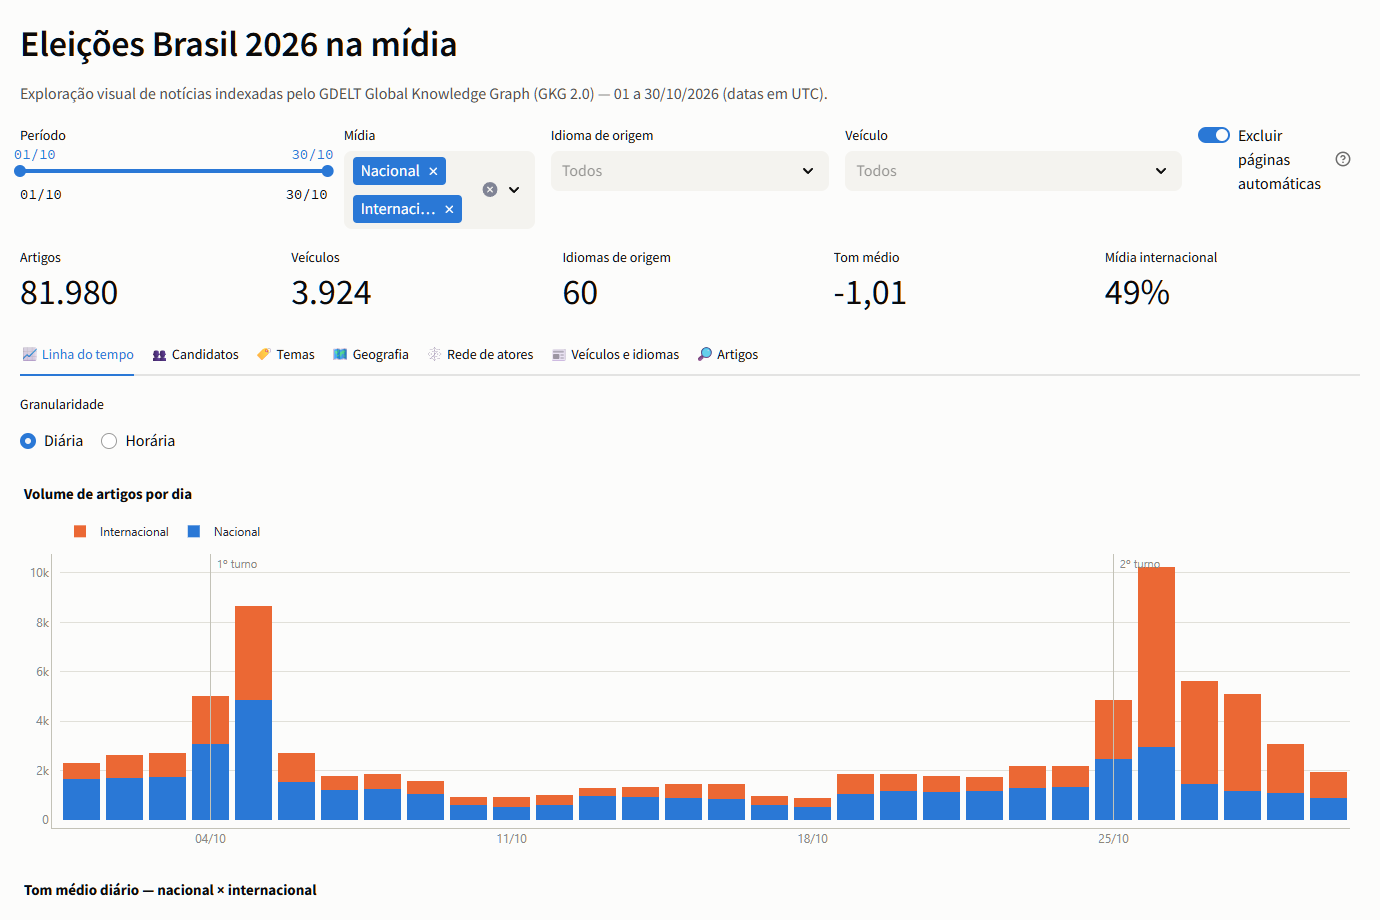
\includegraphics[width=\columnwidth]{dash_visao_geral.png}
  \caption{Tela inicial do painel: filtros globais, indicadores-resumo e a aba \emph{Linha do tempo}.}
  \label{fig:dash}
\end{figure}

%==============================================================
\section{Resultados}\label{sec:resultados}
%==============================================================

\subsection{Conjunto de dados}
Após a remoção de duplicatas restaram 95.403 documentos. Desses, 13.423 (14\%) são páginas automáticas e 81.980 foram analisados. Eles vêm de 3.924 veículos e 60 idiomas de origem: português (42.685), espanhol (14.651), inglês (11.516), alemão (2.084), italiano (1.657) e grego (1.164), entre outros. A mídia internacional responde por 49,1\% dos artigos analisados. Os veículos mais frequentes são \texttt{globo.com}, \texttt{uol.com.br}, \texttt{brasil247.com} e \texttt{revistaforum.com.br}.

\subsection{D1 --- Um artefato de coleta revelado pela visualização}
Na primeira visualização do volume diário, sem filtro, apareceram picos de mais de 11 mil artigos em 5 e 6/10 e de 14 mil em 26/10. Ao mesmo tempo, o \emph{dot plot} de veículos mostrava o \texttt{globo.com} como um ponto muito afastado dos demais, com tom médio $+2{,}16$, enquanto todos os outros grandes veículos ficavam entre $-1{,}1$ e $+0{,}1$. A tabela de artigos (detalhes sob demanda) mostrou a causa: milhares de páginas geradas automaticamente pelo g1, do tipo ``resultado das eleições 2026 em [município]: votação para presidente na [escola] na [n]ª zona eleitoral''. Essas páginas têm tom médio $+3{,}12$, porque são textos curtos cheios de palavras como ``escola'' e ``votação'', e citam os nomes dos candidatos mais votados. A Fig.~\ref{fig:volume} mostra o peso delas (em cinza) nos dias pós-votação. Sem o filtro, essas páginas teriam distorcido três conclusões: o volume nos dias de apuração, o tom da mídia nacional e a visibilidade relativa dos candidatos. Esse resultado ilustra o valor da exploração visual também como ferramenta de \emph{auditoria de dados}.

\begin{figure*}[t]
  \centering
  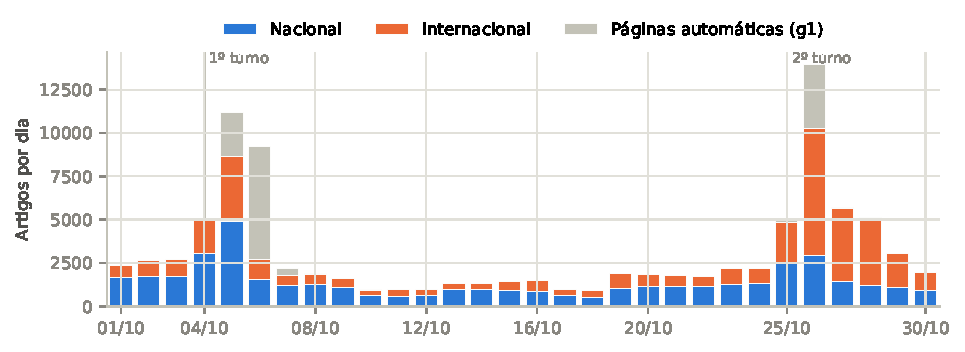
\includegraphics[width=\textwidth]{fig_volume.pdf}
  \caption{Volume diário de artigos por tipo de mídia. Em cinza, as páginas automáticas de resultado por seção eleitoral do g1, excluídas das demais análises.}
  \label{fig:volume}
\end{figure*}

\subsection{D2 --- Ritmo da cobertura (Q1)}
Sem as páginas automáticas, o volume segue dois ciclos bem definidos (Fig.~\ref{fig:volume}). A cobertura sobe a partir do dia da votação, atinge o máximo no dia seguinte a cada turno (5/10 e 26/10, com 10.230 artigos neste último) e decai rapidamente. Entre os turnos, o volume fica em cerca de 1.000 a 2.000 artigos por dia, com degraus nos fins de semana. O 2º turno gerou muito mais cobertura internacional que o 1º: na fase 25--26/10, 64\% dos artigos são estrangeiros, contra 42\% em 4--6/10. A atenção internacional também se manteve alta nos dias seguintes, que concentram 71\% de artigos estrangeiros.

\subsection{D3 --- A mídia internacional é mais negativa (Q2)}
O tom médio da mídia nacional ($-0{,}45$) é mais alto que o da internacional ($-1{,}58$) em \emph{todos} os dias do período (Fig.~\ref{fig:tom}). A diferença é estatisticamente significativa (Mann--Whitney, $p<10^{-3}$) e tem efeito moderado ($d=0{,}45$). Os dois tipos de mídia se aproximam do tom neutro nos dias de votação, quando a cobertura é mais procedimental (comparecimento, apuração), e se tornam mais negativos nos períodos de campanha e no pós-eleição. Por idioma (Fig.~\ref{fig:idiomas}), as coberturas em francês ($-2{,}60$), alemão ($-2{,}06$) e inglês ($-1{,}94$) são as mais negativas. As coberturas em russo ($-0{,}67$) e espanhol ($-1{,}15$) são as menos negativas entre as estrangeiras.

\begin{figure}[t]
  \centering
  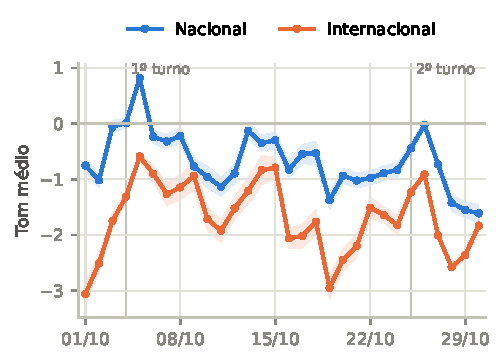
\includegraphics[width=\columnwidth]{fig_tom_midia.pdf}
  \caption{Tom médio diário por tipo de mídia (faixa: IC de 95\%).}
  \label{fig:tom}
\end{figure}

\begin{figure}[t]
  \centering
  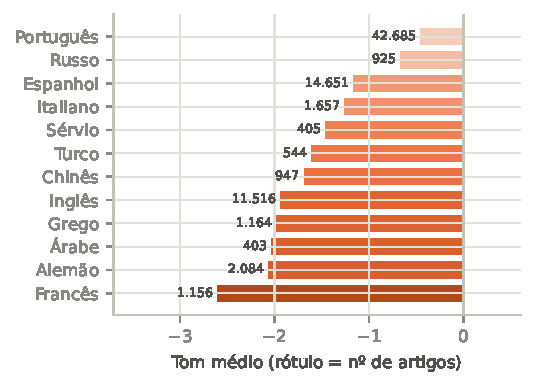
\includegraphics[width=\columnwidth]{fig_idiomas.pdf}
  \caption{Tom médio por idioma de origem (12 idiomas mais frequentes).}
  \label{fig:idiomas}
\end{figure}

\subsection{D4 --- Atores: visibilidade, tom e viés de detecção (Q3)}
Os atores mais citados são Flávio Bolsonaro (27.325 artigos), Lula (26.631), Jair Bolsonaro (12.751) e Donald Trump (8.516). Candidatos derrotados no 1º turno, como Ronaldo Caiado, Romeu Zema e Renan Santos, aparecem em menos de 600 artigos cada. A visão de \emph{fonte da detecção} (Fig.~\ref{fig:atores_tom}b) revelou um viés importante: apenas 17\% das menções a Lula vêm do campo \texttt{V2Persons}, contra 99\% das menções a Jair Bolsonaro. O reconhecedor de entidades do GDELT identifica mal o nome mononímico ``Lula''. Uma análise baseada apenas nesse campo concluiria, erroneamente, que Lula foi cinco vezes menos citado que Flávio Bolsonaro. Pelo mesmo motivo, as menções nacionais a Jair Bolsonaro (119) estão claramente subestimadas, pois a imprensa brasileira costuma escrever apenas ``Bolsonaro''.

A Fig.~\ref{fig:atores} mostra que Flávio Bolsonaro liderou a visibilidade no 1º turno, enquanto Lula dominou o pico do 2º turno (26/10). Nos dias seguintes, Flávio volta a liderar, num movimento ligado à cobertura do pós-eleição (D6). Quanto ao tom (Fig.~\ref{fig:atores_tom}a), Lula tem a cobertura menos negativa entre os quatro atores nas duas mídias. Trump tem a mais negativa na imprensa internacional ($-2{,}15$). A diferença entre mídias é maior para Trump e Flávio Bolsonaro.

\begin{figure*}[t]
  \centering
  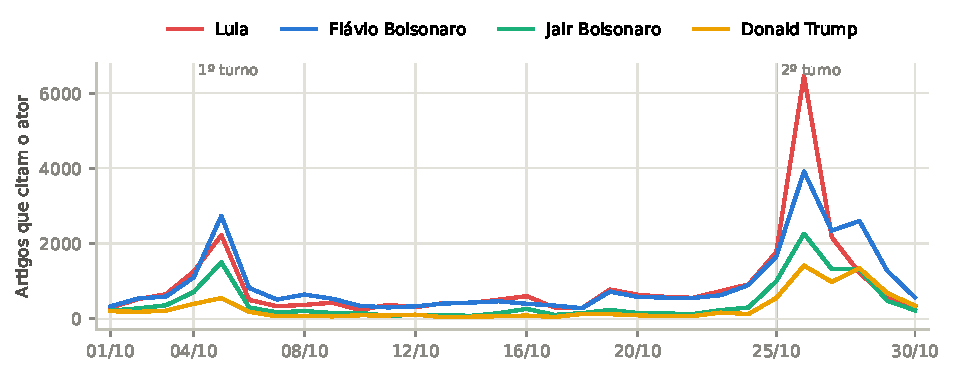
\includegraphics[width=\textwidth]{fig_atores.pdf}
  \caption{Número diário de artigos que citam cada ator (pessoa em \texttt{V2Persons} normalizada \emph{ou} nome na URL).}
  \label{fig:atores}
\end{figure*}

\begin{figure*}[t]
  \centering
  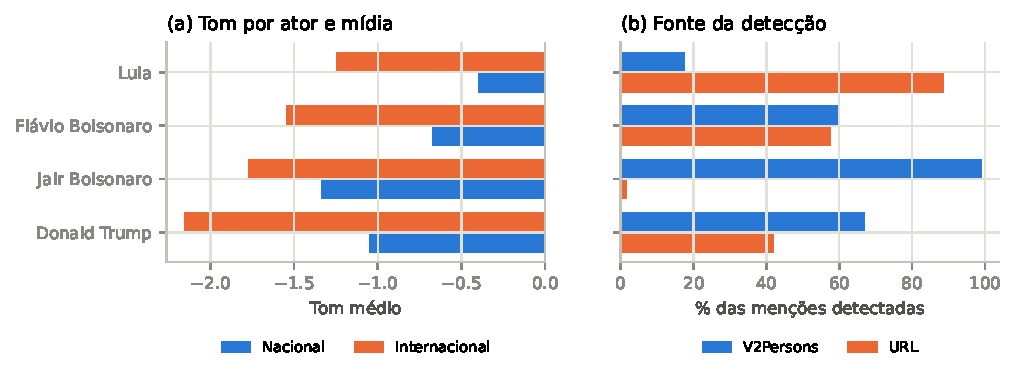
\includegraphics[width=0.85\textwidth]{fig_atores_tom.pdf}
  \caption{(a) Tom médio dos artigos que citam cada ator, por tipo de mídia. (b) Percentual das menções detectadas por \texttt{V2Persons} e pela URL; a soma passa de 100\% porque um artigo pode ser detectado pelas duas vias.}
  \label{fig:atores_tom}
\end{figure*}

\subsection{D5 --- Agenda temática por fase (Q4)}
O mapa de calor tema $\times$ fase (Fig.~\ref{fig:temas}) mostra a agenda se deslocando ao longo do ciclo. Antes do 1º turno e nos dias de votação predominam temas programáticos e procedimentais, como Educação (possivelmente inflado também pelas escolas que servem de locais de votação) e Emprego. Entre os turnos crescem Economia (24\%) e Preços (20\%). No 2º turno, Democracia atinge seu máximo (32\%) e Extremismo, Liberdades políticas e Corrupção também sobem. A série diária mostra ainda um degrau de Corrupção em 19/10, que coincide com o primeiro debate do 2º turno e com a troca de desafios sobre quebra de sigilos bancários entre os candidatos, segundo as URLs desse dia.

O tom por tema é coerente com a semântica de cada um: Fraude eleitoral ($-2{,}84$), Ataque cibernético, Crime e Corrupção ($-2{,}47$) são os mais negativos, enquanto Educação, Emprego e Apoiadores estão perto de $-1$. O tema \texttt{UNGP\_FORESTS\_RIVERS\_OCEANS} aparece em 30--45\% dos artigos em todas as fases. Isso provavelmente é um artefato do classificador, que confunde ``Rio'' (de Janeiro, Grande do Sul etc.) com rios; o tema deve, portanto, ser interpretado com cautela.

\begin{figure}[t]
  \centering
  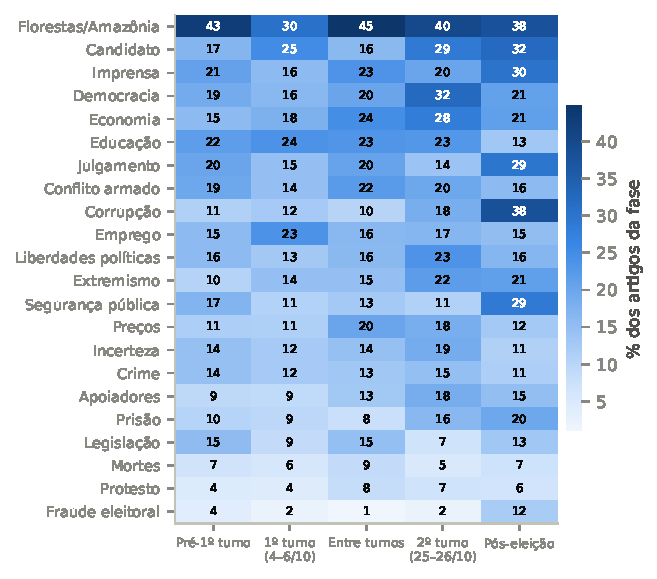
\includegraphics[width=\columnwidth]{fig_temas_fase.pdf}
  \caption{Percentual dos artigos de cada fase classificados em cada tema GKG (22 temas mais frequentes, excluído \texttt{ELECTION}).}
  \label{fig:temas}
\end{figure}

\subsection{D6 --- O pós-eleição como evento internacional}
A fase pós-eleição (27--30/10) é a mais negativa de todo o período: $-2{,}25$ na mídia internacional e $-1{,}27$ na nacional. Ela também é dominada pela imprensa estrangeira (71\% dos artigos). O tema Corrupção salta de cerca de 15\% para 46\% dos artigos em 28/10. Fraude eleitoral passa de 2\% para 12\%, e Julgamento, Prisão e Segurança pública também atingem seus máximos. Pela tabela de detalhes, esses artigos tratam majoritariamente da reação ao resultado do 2º turno: manchetes relatam a reeleição de Lula, a contestação do resultado por Flávio Bolsonaro (que, segundo diversas manchetes, se declarou ``presidente eleito''), a ida dele aos Estados Unidos e declarações de Donald Trump sobre suposta fraude. Isso explica por que Trump, presente em 90\% dos casos em mídia estrangeira, atinge seu pico de citações nessa fase (3.342 artigos)\footnote{Os fatos citados nesta subseção resumem o que a cobertura indexada pelo GDELT reporta, conforme as manchetes das URLs. Resultados oficiais devem ser consultados no TSE.}.

\subsection{D7 --- Rede de atores e geografia (Q5)}
O grafo de coocorrência das 35 pessoas mais citadas, com peso mínimo de 40 artigos em comum (Fig.~\ref{fig:rede}), tem 31 nós e 125 arestas em seu maior componente. O núcleo é formado por Jair Bolsonaro (grau 25), Flávio Bolsonaro (24), Trump (22) e Lula (21), cercados por líderes estrangeiros como Javier Milei, Claudia Sheinbaum, Vladimir Putin e Benjamin Netanyahu. Isso mostra que a eleição foi enquadrada internacionalmente na geopolítica das Américas. Michelle Bolsonaro tem a maior centralidade de intermediação (0,31): ela conecta o núcleo a uma periferia de atores do Congresso e do Judiciário, como Simone Tebet, Davi Alcolumbre, Deltan Dallagnol e André Mendonça.

No mapa (Fig.~\ref{fig:mapa}), São Paulo (16.130 artigos), Distrito Federal (13.737) e Rio de Janeiro (7.799) concentram as menções. O DF aparece por sediar o TSE, o STF e o Executivo federal. Pernambuco tem o maior saldo de menções favorável a Lula ($+0{,}20$) entre as UFs mais citadas, enquanto o DF é o único dos dez primeiros com saldo favorável a Flávio ($-0{,}08$). Fora do Brasil, os países mais mencionados junto à eleição são Estados Unidos (25.401 artigos), Argentina (12.552) e Reino Unido (5.432).

\begin{figure}[t]
  \centering
  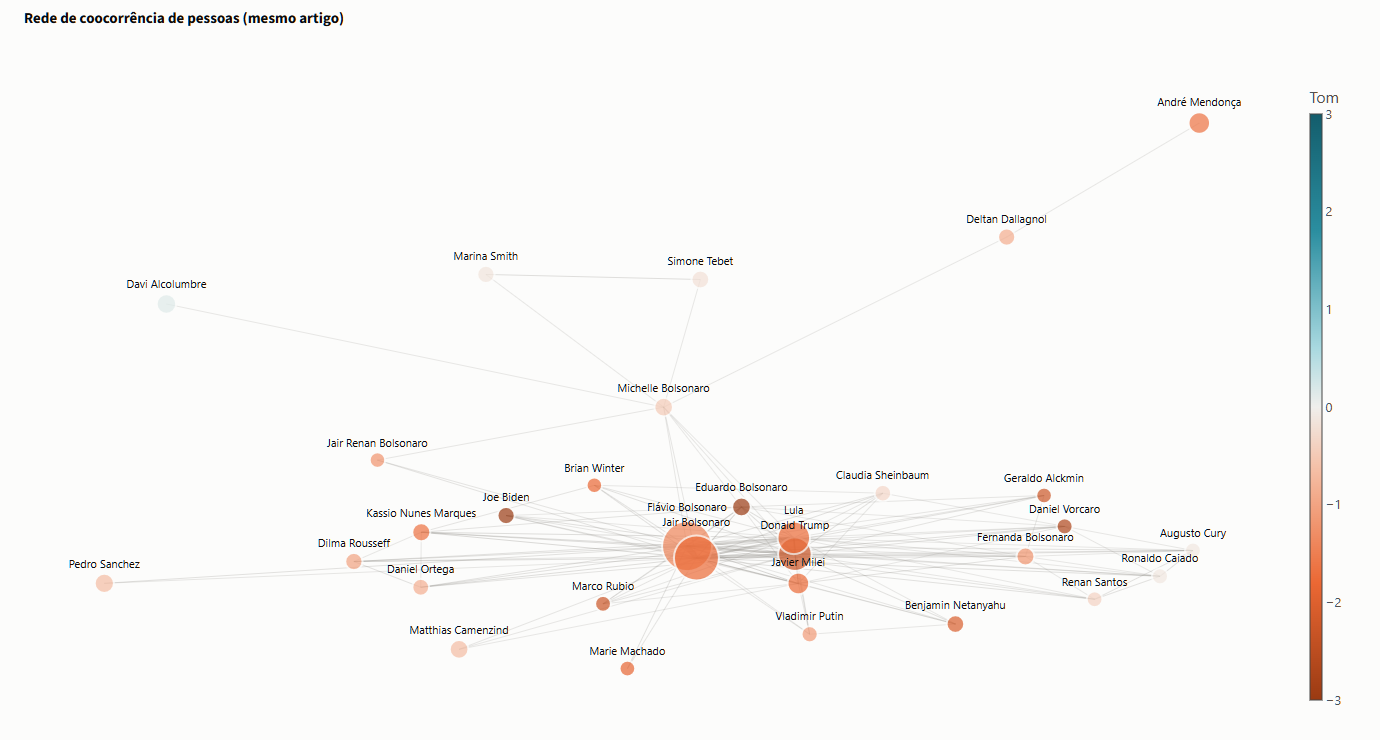
\includegraphics[width=\columnwidth]{dash_rede.png}
  \caption{Rede de coocorrência de pessoas (painel). Tamanho: nº de artigos; cor: tom médio; espessura: nº de artigos em comum.}
  \label{fig:rede}
\end{figure}

\begin{figure}[t]
  \centering
  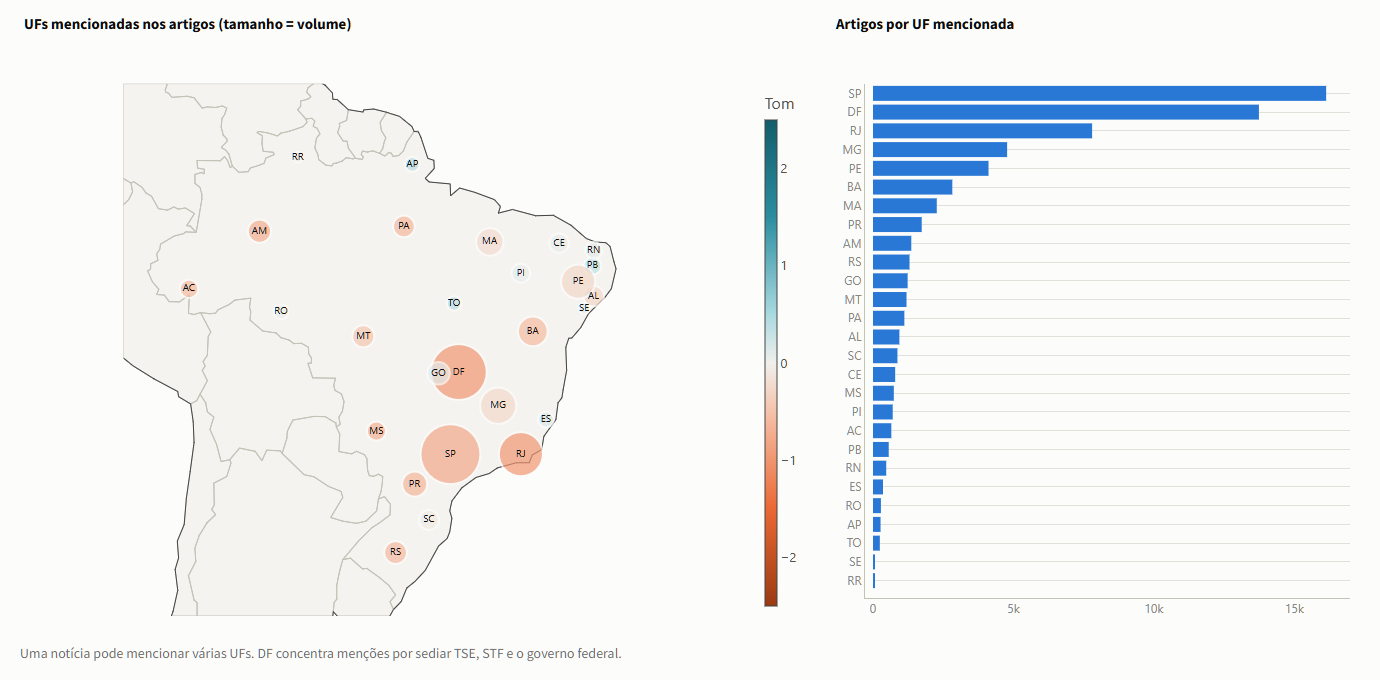
\includegraphics[width=\columnwidth]{dash_mapa.png}
  \caption{UFs mencionadas (painel): área proporcional ao nº de artigos, cor pelo tom médio, e ranking de UFs.}
  \label{fig:mapa}
\end{figure}

%==============================================================
\section{Conclusões}\label{sec:conc}
%==============================================================
Este trabalho desenvolveu um painel de exploração visual interativa para quase cem mil notícias do GDELT GKG sobre as eleições brasileiras de 2026. O painel combina séries temporais, mapas de calor, mapa de símbolos proporcionais, grafo de coocorrência e tabelas sob demanda, todos coordenados por filtros globais. As principais descobertas foram:
(i) a existência de um artefato de coleta (14\% dos registros) que distorcia volume, tom e visibilidade, detectado pela combinação de visões agregadas com detalhes sob demanda;
(ii) um viés sistemático do reconhecimento de entidades contra o nome ``Lula'', corrigido pela combinação de \texttt{V2Persons} com a URL;
(iii) um tom consistentemente mais negativo da imprensa internacional;
(iv) uma agenda que migra de temas programáticos para democracia, corrupção e fraude à medida que a disputa avança; e
(v) um pós-eleição tratado como evento internacional, centrado na contestação do resultado e no envolvimento dos Estados Unidos.

As \textbf{limitações} decorrem principalmente da natureza automática dos dados. O tom é uma medida lexical aplicada, em geral, sobre traduções automáticas, e não distingue a quem o sentimento se dirige. Nomes e temas sofrem erros de tradução e de classificação. A cobertura do GDELT não é uma amostra representativa da imprensa. Por fim, a classificação nacional/internacional baseada em domínio e idioma é aproximada. Como \textbf{trabalhos futuros}, sugerem-se: usar as dimensões emocionais do campo \texttt{GCAM}; detectar mudanças de padrão automaticamente nas séries; analisar o tom no nível das frases que mencionam cada ator; e comparar com as eleições de 2018 e 2022.

\begin{thebibliography}{00}
\bibitem{card1999} S. K. Card, J. D. Mackinlay e B. Shneiderman, \emph{Readings in Information Visualization: Using Vision to Think}. San Francisco: Morgan Kaufmann, 1999.
\bibitem{munzner2014} T. Munzner, \emph{Visualization Analysis and Design}. Boca Raton: CRC Press, 2014.
\bibitem{shneiderman1996} B. Shneiderman, ``The eyes have it: A task by data type taxonomy for information visualizations,'' in \emph{Proc. IEEE Symp. Visual Languages}, 1996, pp. 336--343.
\bibitem{keim2002} D. A. Keim, ``Information visualization and visual data mining,'' \emph{IEEE Trans. Vis. Comput. Graphics}, vol. 8, no. 1, pp. 1--8, 2002.
\bibitem{heer2012} J. Heer e B. Shneiderman, ``Interactive dynamics for visual analysis,'' \emph{Commun. ACM}, vol. 55, no. 4, pp. 45--54, 2012.
\bibitem{harrower2003} M. Harrower e C. A. Brewer, ``ColorBrewer.org: An online tool for selecting colour schemes for maps,'' \emph{The Cartographic Journal}, vol. 40, no. 1, pp. 27--37, 2003.
\bibitem{fruchterman1991} T. M. J. Fruchterman e E. M. Reingold, ``Graph drawing by force-directed placement,'' \emph{Software: Practice and Experience}, vol. 21, no. 11, pp. 1129--1164, 1991.
\bibitem{clauset2004} A. Clauset, M. E. J. Newman e C. Moore, ``Finding community structure in very large networks,'' \emph{Physical Review E}, vol. 70, 066111, 2004.
\bibitem{leetaru2013} K. Leetaru e P. A. Schrodt, ``GDELT: Global data on events, location, and tone, 1979--2012,'' in \emph{ISA Annual Convention}, 2013.
\bibitem{mckinney2010} W. McKinney, ``Data structures for statistical computing in Python,'' in \emph{Proc. 9th Python in Science Conf.}, 2010, pp. 56--61.
\bibitem{hagberg2008} A. A. Hagberg, D. A. Schult e P. J. Swart, ``Exploring network structure, dynamics, and function using NetworkX,'' in \emph{Proc. 7th Python in Science Conf.}, 2008, pp. 11--15.
\bibitem{hunter2007} J. D. Hunter, ``Matplotlib: A 2D graphics environment,'' \emph{Computing in Science \& Engineering}, vol. 9, no. 3, pp. 90--95, 2007.
\end{thebibliography}

\end{document}
